\RequirePackage[l2tabu, orthodox]{nag}
%\documentclass[a4paper,12pt]{article}
\documentclass[man,floatsintext]{apa6} % man, doc, jou

\usepackage{amsmath}
% \usepackage[a4paper]{geometry}
\usepackage{graphicx}
\usepackage{microtype}
\usepackage{siunitx}
\usepackage{booktabs}
\usepackage{apacite}
% \usepackage{natbib}
%\usepackage{newclude} % \include* to include without page break
%\usepackage[colorlinks=false, pdfborder={0 0 0}]{hyperref}
\usepackage{cleveref} % \cref instead of \ref, automatic "Section" etc.
\usepackage{eurosym}

\setlength{\parskip}{0cm plus0mm minus0mm}

\graphicspath{ {./figures/} }

\title{Predicting reaction time using oscillations in the beta band}
\shorttitle{Predicting reaction time with beta activity}
\author{
  Max Hollmann

  (s2180812)
}
\affiliation{
  \vspace{1cm}
  \today
  \vspace{1cm}

  Bachelor Thesis BSc Programme of Psychology

  Faculty of Behavioural and Social Sciences

  University of Groningen

  \vspace{1cm}
  Supervised by: Dr. Hedderik van Rijn

  Secondary evaluator: Udo Boehm

  In collaboration with: Simon Kock, Niklas Fasching, and Robbert van der Mijn
}
\date{\today}
\authornote{Thanks to Dr. Hedderik van Rijn, Dr. Mark Span, Udo Boehm, Dr. Jacob Jolij, and Prof. Dr. Ritske de Jong for their assistance on this project.}

\abstract{Interval timing plays a role in reaction time experiments,
  in that it creates anticipation effects when stimuli occur after a
  predictable interval, which when altered leads to predictable
  changes in response speed.

  An index of interval timing processes that emerged in the recent
  years is beta activity, which has been found to play a role in
  interval timing tasks via motor preparation.

  The present study deals with the question whether beta activity can
  thus be used to predict response speed. Beta activity was measured
  during the foreperiods of a simple reaction time task and looked at
  as a potential predictor of response speed.

  Results confirm the finding that deviations from the expected
  pre-stimulus interval influence response speed as expected, but
  clearly show beta activity to be non-predictive. This is in line
  with brain imaging studies that revealed different neural structures
  to be responsible for implicit and explicit timing tasks.}

\keywords{beta power, interval timing, reaction
  time, variable foreperiods}

\begin{document}
\maketitle
The passage of time is one of the most basic facts of our world,
making timing one of the most important functions of the mind.  Thus,
a lot of scientific effort is spent on discovering its underlying
mechanisms.

One line of research in this area is looking at connections between
electrophysiological measures from the brain and interval timing.  For
example, \citeA{macar_supplementary_1999} found a positive correlation
between the amplitude of a negative cortical potential during a
self-produced interval and the duration of the same interval.
However, in a replication of this experiment
\citeA{kononowicz_slow_2011} failed to find the same effect.

More recently, the power of neuronal oscillations in the beta band was
found to be another measure that is predictive of the length of
produced intervals. \citeA{jenkinson_new_2011} suggested that beta
power in the basal ganglia provides an index of the likelihood that a
voluntary movement will be required, with a low beta power indicating
a high probability.  Indeed, \citeA{joundi_persistent_2013} found that
in a task where participants were instructed to tap along with an
external rhythm, beta power was lower during the tapping than at
baseline. Furthermore, they found that with high tapping rates, beta
activity could not fully resynchronize between
taps.

Along similar lines, \citeA{bartolo_information_2014} used beta power
to predict the interval length in a synchronization-continuation
tapping task performed on monkeys.  In this experiment subjects first
tapped along with an externally provided beat (synchronization), and
then continued tapping at the same speed without external guidance
(continuation).  During the continuation part longer intervals were
associated with higher beta power during the interval, and vice versa.

\citeA{kononowicz_beta_2014} extended these findings to an interval
production task in humans in which participants were instructed to
estimate time intervals of 2.5 seconds by pressing a key twice.  In
this study intervals were distinct from each other, providing a clear
association between the beta power measured during the interval and
the length of the interval itself, and also provided enough time for
beta oscillations to fully resynchronize between trials.  As in
\citeauthor{bartolo_information_2014}'s study, beta power was
positively correlated with the length of the produced intervals.

In another area of the field of timing, a large body of research
exists that links interval timing to reaction time tasks
\cite<e.g.,>{karlin_reaction_1959, drazin_effects_1961,
  grosjean_timing_2001}.  When participants come to expect the trigger
stimulus after a specific time interval, deviations from this interval
lead to predictable changes in reaction time.  For example,
\citeA{grosjean_timing_2001} found that when the stimulus appears
earlier than expected, reaction times will be slower.  Conversely,
when it appears later than expected, reaction times will be faster.  A
straightforward explanation for this effect is that participants build
up the readiness to react towards the point in time when they expect
the stimulus to occur.  When it appears before they expect it, they
are less ready to respond to it, and thus slower.  However, for
stimuli that appear later than anticipated, the readiness is very high
and the reaction comes faster. These findings clearly show that timing
plays a role in reaction time tasks, in that participants implicitly
use their sense of time to predict when the stimulus will occur.

The purpose of the present study is to investigate the link between
beta power, interval timing, and reaction time.  As beta power has
been found to increase the length of estimated time intervals
\cite<e.g.>{kononowicz_beta_2014}, and interval timing has been shown
to play a role in reaction time tasks via expectancy effects
\cite<e.g.>{grosjean_timing_2001}, we hypothesize that beta power can
be used to predict the expectancy, and hence the response speed, in a
reaction time task.

To assess this hypothesis, we performed a simple reaction time task in
which participants initiated each trial themselves by pressing a key.
Beta power was measured during the first second of each trial.  For
the first 150 trials, the trigger stimulus always occurred after a 1.8
s from the start of the trial, in order for subjects to come to expect
the stimulus after this interval.  In the last 250 trials, the
interval was chosen at random from the standard interval, and both 100
ms longer and shorter intervals.  The interval lengths were chosen
such that enough time passed between start of the trial and stimulus
onset to allow the beta power to build up to its peak within the
interval \cite<see>{kononowicz_beta_2014}.

In line with the findings of \citeA{grosjean_timing_2001}, reaction
times were hypothesized to be slower for the shorter interval, and
faster on trials with the longer interval. In addition, we expected
reaction times to be faster in trials where beta power is low, because
participants hypothetically estimate the interval to end sooner than
it actually does, and are thus very ready to respond when the stimulus
finally does occur.  Conversely, in trials with high beta power,
participants should estimate the stimulus to occur later than it does,
and thus not be prepared for it when it actually occurs, leading to a
slower reaction time.

\section{Method}
\subsection{Participants}
36 English speaking international students at the University of
Groningen (14 male) participated in the study, with ages ranging from
19 to 25 ($M = 21.86$, $SD = 1.71$). Ten participants received partial
course credits, while the remaining 26 were recruited via
advertisements on a social network and received \euro 5 for
participation. Four participants were excluded since EEG data was
missing. One further participant was excluded due to a dysfunctional
keyboard.

\subsection{Electrophysiological Recording and Materials}
The EEG signal was sampled at 250 Hz at a resolution of 71.5 nV/bit
using a Porti 16 channel amplifier (TMS International BV) with an
analog anti-aliasing filter set to a cutoff frequency of 125 Hz. Five
locations on the scalp (Cz, Fz, Pz, C3, and C4 according to the
international 10-20 system) were measured using an EEG cap
(Electro-Cap International, Inc.). Furthermore, vertical (measured on
the left eye) and horizontal eye movements, as well as the mastoids
(A1, A2) were recorded. All electrodes were made of tin and their
impedances kept below 10 k$\Omega$.

Signals were referenced to the average of both mastoid
electrodes. Power in the beta band (15-30 Hz) was computed from the
five scalp electrodes during the first second of the interval, tapered
with a 40\% Hanning window, using a fast Fourier transform.

The experimental code was written in MATLAB (version R2011b, 32 bit,
MathWorks) running on Windows XP, making use of the Psychtoolbox
library (http://psychtoolbox.org). Responses were recorded using a PS2
keyboard with a polling rate above 200 Hz. A 27'' monitor (iiyama
ProLite G2773HS; $1920 \times 1080$ pixels, 120 Hz) was employed.

\subsection{Data preprocessing}
Raw EEG data was filtered offline with a band-pass filter using 1-40
Hz, as well as a 49-51 Hz notch filter to remove noise from electronic
devices in the room.

For every participant, the last 22 trials were excluded due to a
technical issue, as well as the trials that had beta values outside
the range of three standard deviations. Trials containing eye
movements in the horizontal or vertical channels were
excluded. Additionally, trials containing artifacts were excluded after
visual inspection.

Based on \citeA{grosjean_timing_2001}, trials with a negative reaction
time or a reaction time exceeding 1000 milliseconds were not included
in the analyses. On average 98.61 trials ($SD = 42.72$) were removed
for each participant.

\subsection{Task and Stimuli}
Before the beginning of the experiment, participants were instructed
not to use any timing aids (e.g., counting) and not to move or blink
their eyes during trials. Each trial consisted of the following
sequence of events, all presented on a black background. First, a
reminder to blink (``Please blink!'', white letters on a black
background) was presented for 1500 ms. This was followed by a gray
fixation circle. Participants started the interval by pressing the
spacebar. The circle turned white immediately after the spacebar was
pressed, and stayed white until the end of the trial. The length of
the interval differed between conditions and was not explicitly
communicated to participants. At the end of the interval a target
sound (1000 Hz, 0.2 s) was played to which participants were
instructed to react to as quickly as possible by pressing the spacebar
a second time. The reaction time was recorded as the time between the
onset of the sound stimulus and the second key press.

Feedback for valid responses was given on a 5-point scale represented
by a row of five circles (see \Cref{fig:task}). Responses preceding
the sound onset were given feedback in the form of the text ``too
early'' displayed in red. All visual elements were displayed centrally
on the screen to minimize eye-movement artifacts in the EEG signal.

\begin{figure}[!h]
  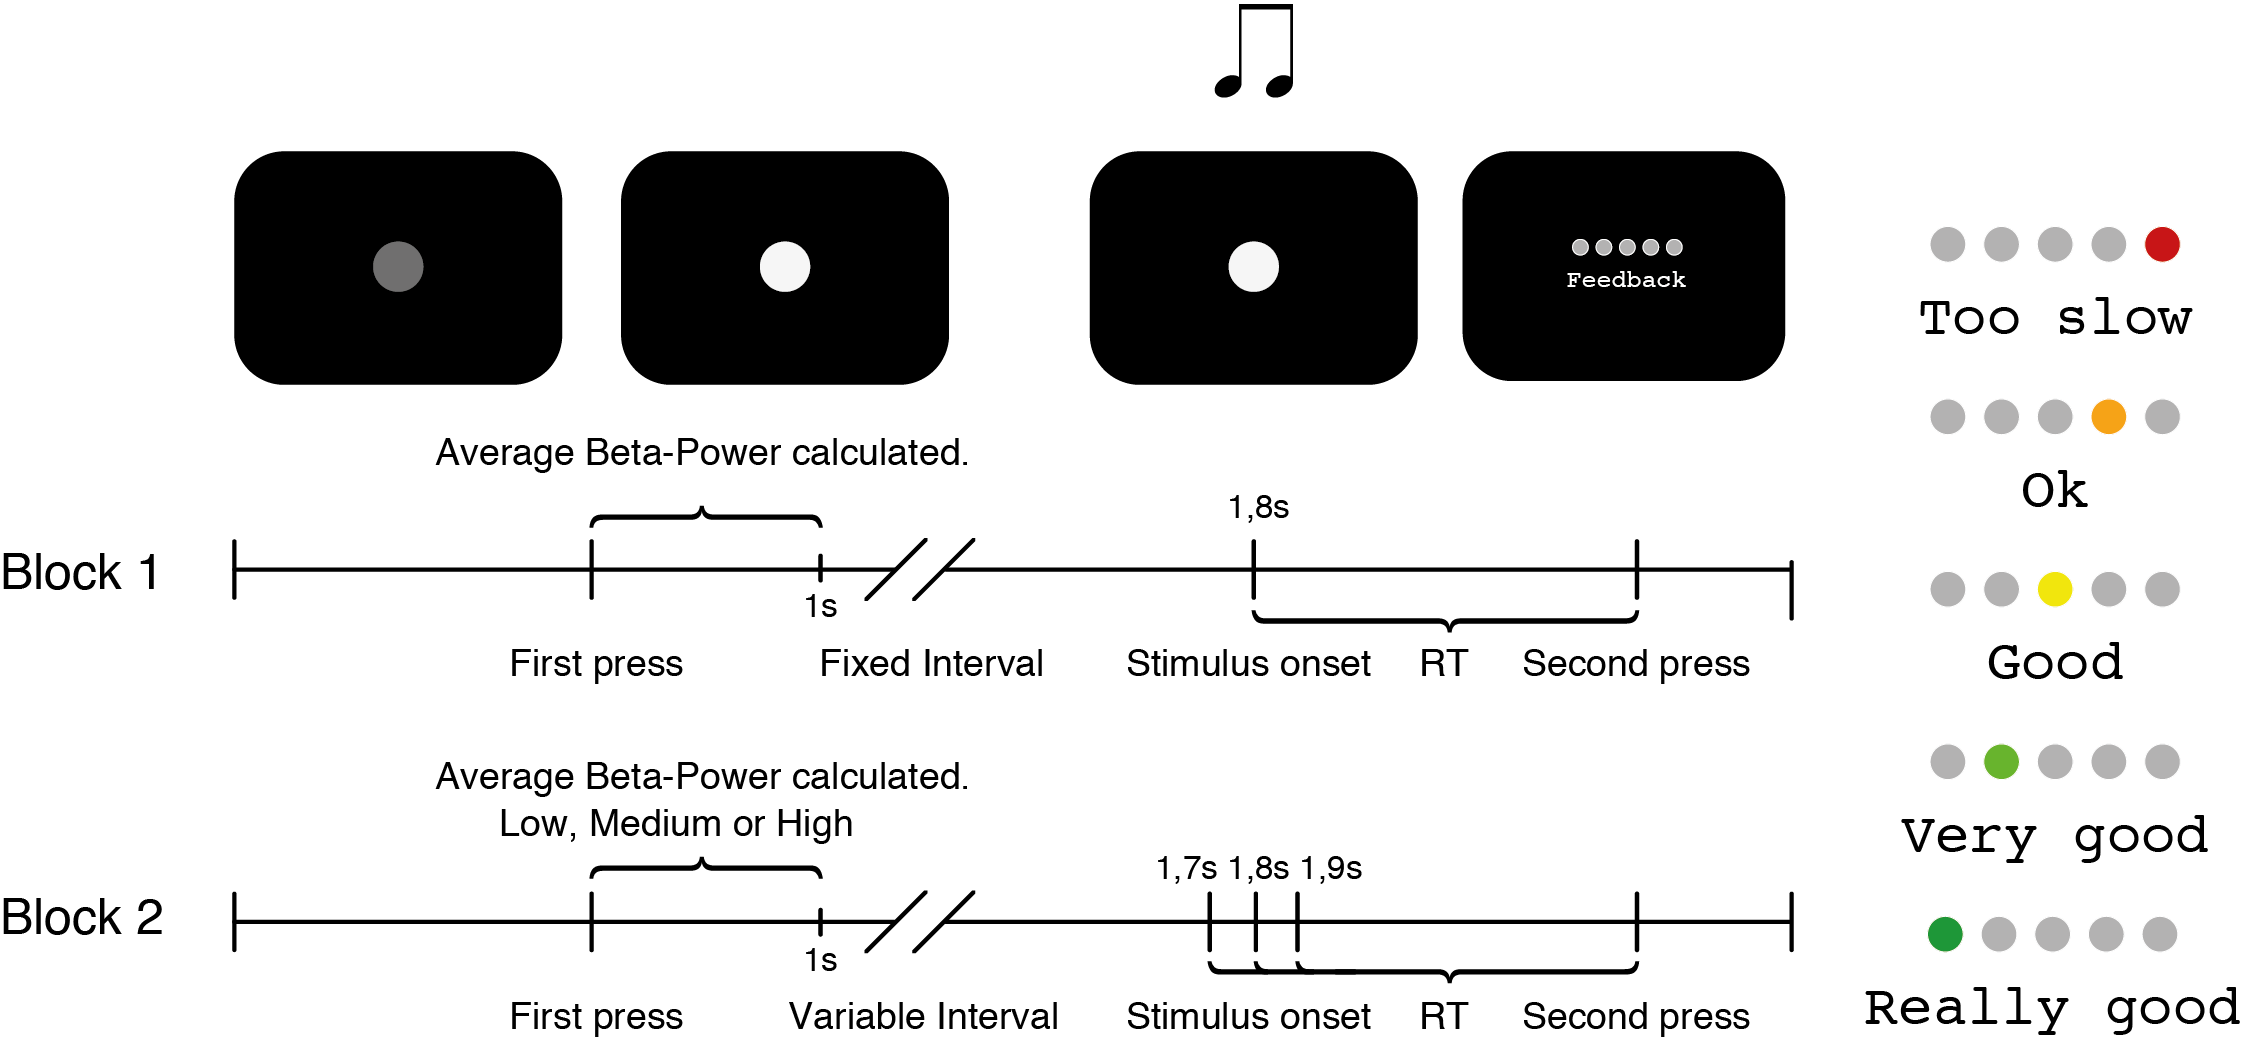
\includegraphics[width=\textwidth]{trial}
  \caption{Sequence of events in one trial.}
  \label{fig:task}
\end{figure}

\subsection{Design}
For this experiment a within-subjects design was used. The dependent
variable was reaction time to the onset of a tone, presented after a
certain interval. The independent variable in the quasi-experimental
Block 1 was average beta power during the first second of the
trial. During experimental Block 2, besides beta power in the first
second of the interval, the length of the presented interval was of
interest as well. The length condition was varied randomly within
participants, as described below.

\subsection{Procedure}
The experiment was split into two experimental blocks preceded by five
practice trials. Every 105 trials the participants were presented a
screen instructing them to take a break.

Block 1 consisted of 150 trials with an invariant interval of 1.8
seconds (see \Cref{fig:task}). The primary purpose of this block was
to acquaint the participants with this interval and get them to expect
it in later trials. The data from Block 1 was also used to create an
initial distribution of the beta power for the BCI component,
described below.

In the second block of the experiment participants completed 250
trials. Contrary to Block 1 the interval length was not fixed, but for
each trial drawn from three conditions: short (1.7 seconds), standard
(1.8 seconds) and long (1.9 seconds) (see \Cref{fig:task}).

\subsubsection{Brain Computer Interface}
A brain computer interface (BCI) setup was used to facilitate an
optimal distribution of length conditions according to the average
beta power during the first second of the interval. More specifically,
to obtain a higher number of non-average beta values in trials with
non-standard interval lengths. Therefore, the distribution of beta
power of all previous trials was updated with the beta power of the
current trial and then split into three parts (lower $^2/_5$,
middle $^1/_5$, and upper $^2/_5$). The beta power in the
current trial was then categorized according to that distribution.

For an average beta value (the middle $^1/_5$ of the
distribution) participants were always shown the standard
interval. For a high beta value (upper $^2/_5$ of the
distribution) participants were presented one of the three conditions,
determined by randomly drawing (without replacement) from a list that
contained five short, five long, and two standard intervals. This
procedure ensured that each condition was presented randomly, but also
approximately equally frequent across participants. When the list was
empty (i.e. after 12 beta values in the high condition) a new list was
created. A low beta value (lower $^2/_5$ of the beta
distribution) was handled in the same manner as a high beta value,
though an independent but identical list was used.



\section{Results}
The hypotheses were that participants react slower if the stimulus is
presented earlier and faster if the stimulus is presented later
compared to the standard interval after which the stimulus is
presented (1), and that participants with a higher beta power in the
first second of the interval produce slower reaction times and vice
versa (2).

\subsection{BCI}
Due to the calculation of the beta power being implemented
incorrectly, the BCI component of the setup did not provide the
intended benefit of an ideal distribution of beta power across length
conditions. Beta power was recalculated from the EEG signal for the
subsequent analysis.

\subsection{Assumptions}
Due to the repeated measures nature of the research design,
observations were not independent. To control for between-subject as
well as time series effects in the reaction times, the effects of
subject and trial number as well as their interaction were partialed
out. More specifically, we used the residuals of a linear regression
with subject and trial number as predictors for reaction time.

Normality of the data could not be assumed since reaction times were
found to be right skewed ($skewness = 1.57$, $kurtosis =
18.05$). Moreover linearity assumptions did not hold for either
independent variable. However, homoscedasticity could be assumed. Even
though some assumptions were violated, the linear regression model was
used.

\subsection{Linear Regression}
To test the hypotheses a linear regression was performed predicting
reaction time from length condition, beta power, and their interaction
(\Cref{tbl:regression}). Descriptive statistics of the data are
provided in \Cref{tbl:descriptives}.

In comparison to the reaction times in the medium length condition ($M
= 0.188$, $SD = 0.061$), reaction times in the long condition were on
average 17.1 ms faster ($t(9480) = -10.438$, $p < .001$) while
reaction times in the short condition were on average 25.9 ms slower
($t(9480) = 16.93$, $p < .001$), these results are in line with first
hypothesis (\Cref{fig:rt_by_length}).

However, neither beta as main effect ($t(9480) = -0.493$, $p = 0.622$)
nor the interaction between beta and length condition were found to
have a significant effect on reaction time ($t(9480) = 0.658$, $p =
0.51$ for beta on short compared to medium condition; $t(9480) =
-0.641$, $p = 0.52$ for beta on long compared to medium
condition). Thus no evidence was found to support our second hypothesis
(\Cref{fig:rt_by_beta}).

\begin{figure}[!h]
  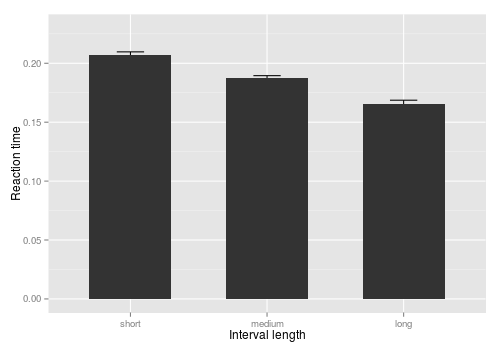
\includegraphics[width=0.7\textwidth]{actual_rt_by_length}
  \caption{Mean reaction time by length condition.}
  \label{fig:rt_by_length}
\end{figure}

\begin{figure}[!h]
  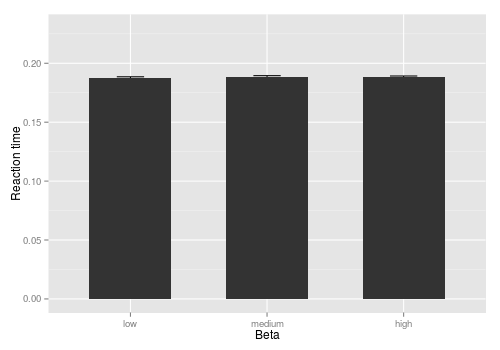
\includegraphics[width=0.7\textwidth]{actual_rt_by_beta}
  \caption{Mean reaction time by beta power (cut-offs at $^1/_3$ and $^2/_3$ quantiles).}
  \label{fig:rt_by_beta}
\end{figure}

\subsection{Bayes Factor Analysis}
As we cannot reject the utility of beta power as a predictor for
reaction time using the conventional linear regression model, we
employed Bayesian statistics to grade the decisiveness of the evidence
\cite{jeffreys_theory_1961}. The \emph{lmBF} function from the R
package \emph{BayesFactor} (version 0.9.7) was used to compare the
full model including both length condition and beta power to a model
including only length condition. The model omitting beta power was
favored with a Bayes factor of 28.99 ($\pm 1.33\%$). According to
\citeA{jeffreys_theory_1961} this Bayes factor can be interpreted as
strong evidence against the model including beta power as a predictor.


\begin{table}[!h]
  \caption{Regression coefficients for the linear model predicting reaction time.}
  \begin{flushleft}
    \begin{tabular}{lrrrr}
      \toprule
                                                    & B        & SE         & t       & p         \\
      \midrule
      Intercept                                     & -0.0029  & 0.0008     &  -3.42  & $< 0.001$ \\
      Length condition: long                        & -0.0171  & 0.0016     & -10.44  & $< 0.001$ \\
      Length condition: short                       &  0.0259  & 0.0015     &  16.96  & $< 0.001$ \\
      Beta power                                    & -0.0031  & 0.0063     &  -0.49  & $0.622$   \\
      Beta power $\times$ Length condition: long    & -0.0079  & 0.0123     &  -0.64  & $0.521$   \\
      Beta power $\times$ Length condition: short   & -0.0086  & 0.0130     &   0.66  & $0.511$   \\
      \bottomrule
    \end{tabular}
  \end{flushleft}
  \label{tbl:regression}
\end{table}

\begin{table}[!h]
  \caption{Means and standard deviations of reaction time and beta power overall and by length conditions. Note that neither beta power nor reaction time are corrected for subject and trial effects.}
  \begin{flushleft}
    \begin{tabular}{lrrrrr}
      \toprule
                               & \multicolumn{2}{l}{Reaction time}              && \multicolumn{2}{l}{Beta}                       \\ \cmidrule{2-3} \cmidrule{5-6}
                               & \multicolumn{1}{l}{M} & \multicolumn{1}{l}{SD} && \multicolumn{1}{l}{M} & \multicolumn{1}{l}{SD} \\
      \midrule
      Overall                  & 0.188                 &  0.067                 && 0.277                 & 0.188                  \\
      Length condition: short  & 0.207                 &  0.070                 && 0.270                 & 0.168                  \\
      Length condition: medium & 0.188                 &  0.061                 && 0.283                 & 0.200                  \\
      Length condition: long   & 0.166                 &  0.070                 && 0.271                 & 0.177                  \\
      \bottomrule
    \end{tabular}
  \end{flushleft}
  \label{tbl:descriptives}
\end{table}


\section{Discussion}
In the present study we investigated the connection between interval
timing, beta power, and reaction time. We tested whether presenting
the stimulus to react to earlier or later than expected would
influence response speed, and in addition, whether beta activity would
influence reaction time by changing the time at which participants
expect the stimulus.

\subsection{Interval Length}
The first of our hypotheses, predicting that reaction times will be
slower in trials with a short interval, and faster in trials with a
long interval, was clearly supported by the data.  With the short and
long intervals leading, respectively, to a 25.9 ms and a 17.1 ms
difference in reaction time to the standard condition, this effect is
very substantial given that the difference between the conditions was
only 100 ms.

As expected from previous studies \cite<e.g.,>{karlin_reaction_1959,
  drazin_effects_1961, grosjean_timing_2001}, participants reacted
slower in trials with short intervals, and faster in trials with long
intervals. The decrease in response speed for short intervals can be
accounted for by the fact that participants are likely not yet
prepared to react, as they do not expect the stimulus to occur at this
time.

The faster response speed on trials with long intervals is more
interesting. It would seem reasonable to expect participants to %
increase their preparedness to react until the point when they expect
the stimulus, and then either stay on that level of preparedness, or
even ``lose interest'' and become slower again. Our findings, however,
suggest that preparedness increases even further after the point in
time when the stimulus is expected to occur. This supports research by
\citeA{naatanen_diminishing_1970}, who argued that the increase in
response speed in fact stems from the passage of time. As participants
know that the stimulus will occur eventually, the more time passes,
the likelier it becomes that it will occur in the next moment
\cite<referred to in the literature as the \emph{hazard rate};
e.g.,>{kononowicz_decoupling_2014}. This perspective leads to the
prediction that reaction time becomes faster the more time elapses
before the stimulus, which is in fact what we found. It would be an
intriguing question for future research over what time span this
effect holds.

It is interesting to note that we obtained similar results as previous
research in spite of significant differences in experimental
design. In \citeA{drazin_effects_1961}'s study, participants were
aware of the different interval durations, while no participant in our
study reported noticing the differences. This makes it clear that the
processes leading to the changes in reaction time do not rely on
conscious perception.

\subsection{Beta Power}
Our second hypothesis, that beta power will correlate positively with
reaction time, was not confirmed.  In fact, Bayesian analyses even
clearly suggested that it did not have any value as a predictor of
reaction time.

This finding can be interpreted using the taxonomy proposed by
\citeA{coull_dissociating_2008}.  \citeA{kononowicz_beta_2014}'s task
required motor timing, a form of explicit timing that has been shown
to be associated with activation of the basal ganglia
\cite{coull_dissociating_2008}.  The present study, in contrast, uses
a task involving implicit timing; more specifically, exogenous
temporal expectations, which involve multiple different brain areas,
but not the basal ganglia \cite{coull_dissociating_2008}.  As the beta
power that is associated with timing functions has been described as
originating from the basal ganglia, and only in studies employing
explicit timing tasks \cite<e.g.,>{joundi_persistent_2013,
  bartolo_information_2014}, it is plausible that beta power does not
index the implicit timing required for the present study.  Thus, our
finding that beta power is not suited as a predictor of reaction time
aligns with the idea proposed by \citeA{coull_dissociating_2008} that
implicit and explicit timing employ different neural structures.

Another possible reason for beta power not being useful to predict
reaction time is that our task differed from those of
\citeA{kononowicz_beta_2014} and \citeA{bartolo_information_2014} in
that it did not allow participants to fully plan when to make the
second key press directly after the first one, as they had to wait for
the stimulus to respond. In other words, while previous tasks required
responses based purely on internal cues (interval timing), the present
task required participants to wait for an external cue to
respond. Thus, our finding might suggest that internally and
externally cued tasks employ different timing mechanisms.

Lastly, the room in which the experiment was run in was not
electrically shielded, resulting in a lot of noise in the EEG signal,
which might have masked the effect. Furthermore, we did not use the
FCz electrode as \citeA{kononowicz_beta_2014} did, but electrodes
surrounding it. Regarding these two issues, however, post-hoc analyses
revealed a significant relationship between subjects' mean beta power
and mean reaction time, indicating that beta activity was measured in
a meaningful way. Moreover, our data did not satisfy all assumptions
of the linear regression model; normality, independence, and linearity
were violated.

\subsection{Brain Computer Interface}
A technical mistake in the implementation of the beta power
calculation led to a long-term drift in the beta values, so that the
BCI algorithm categorized almost all trials as either high or
low. Thus, the BCI did not provide the intended benefit of obtaining
as many non-standard interval lengths on trials with non-average beta
values as possible. Instead, length conditions were distributed
randomly without regard for the beta power in the current trial.
Given the potential benefit of a more beneficial distribution of
conditions, combined with no negative effects in case of failure, the
kind of BCI used in the present study can safely be used in future
research of a similar nature.

\subsection{Conclusion}
We found evidence for an effect of interval length on reaction time,
in line with previous research \cite{naatanen_diminishing_1970,
  karlin_reaction_1959, drazin_effects_1961,
  grosjean_timing_2001}. Beta power, however, was found not to be
suitable as a predictor, which can be explained by brain imaging
studies that found that explicit and implicit timing activates
different brain regions \cite{coull_dissociating_2008}.

\bibliographystyle{apacite}
\bibliography{/home/max/Dropbox/Psychology/Thesis/latex/clean_references}

\end{document}
